Un tablero de ajedrez es una grilla
de ocho filas y ocho columnas, numeradas de 1 a 8.
Dos de las piezas del juego de ajedrez son el alfil y la torre.
El alfil se desplaza en diagonal,
mientras que la torre se desplaza horizontal o verticalmente.
Una pieza puede ser capturada por otra
si está en una casilla a la cual la otra puede desplazarse:

\tikzstyle{pieza}=[circle, inner sep=1pt]
\tikzstyle{ma}=[ultra thick, densely dotted, black!45]
\tikzstyle{mt}=[ultra thick, dashed, black!45]
\def\tablero{%
  \foreach\row in {2,4,...,8}
    \foreach\col in {1,3,...,7}
      \fill[black!20] (\row - .5, \col - .5) rectangle (\row + .5, \col + .5);
  \foreach\row in {1,3,...,7}
    \foreach\col in {2,4,...,8}
      \fill[black!20] (\row - .5, \col - .5) rectangle (\row + .5, \col + .5);
  \draw (.4, .4) rectangle (8.6, 8.6);
  \foreach\row in {1,...,8}
    \node[anchor=east]  at (.4, \row) {\footnotesize\row};
  \foreach\col in {1,...,8}
    \node[anchor=south] at (\col, .4) {\footnotesize\col};
}
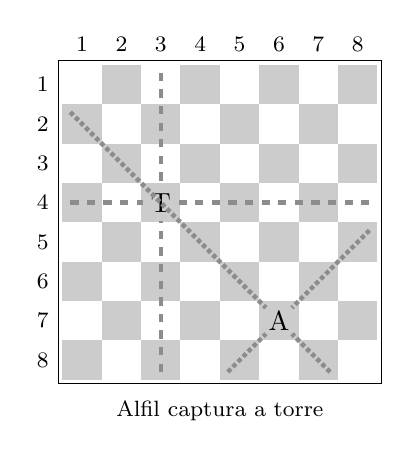
\begin{tikzpicture}[scale=.5, yscale=-1]
  \tablero
  \node[pieza] (alfil) at (6, 7) {A};
  \node[pieza] (torre) at (3, 4) {T};
  \draw[ma] (1 - .3, 2 - .3) -- (alfil);
  \draw[ma] (5 - .3, 8 + .3) -- (alfil);
  \draw[ma] (8 + .3, 5 - .3) -- (alfil);
  \draw[ma] (7 + .3, 8 + .3) -- (alfil);
  \draw[mt] (3     , 1 - .3) -- (torre);
  \draw[mt] (3     , 8 + .3) -- (torre);
  \draw[mt] (1 - .3, 4     ) -- (torre);
  \draw[mt] (8 + .3, 4     ) -- (torre);
  \node at (4.5, 9.3) {\footnotesize Alfil captura a torre};
\end{tikzpicture}
\hfil
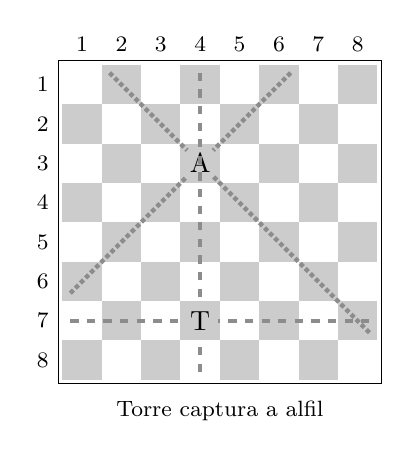
\begin{tikzpicture}[scale=.5, yscale=-1]
  \tablero
  \node[pieza] (alfil) at (4, 3) {A};
  \node[pieza] (torre) at (4, 7) {T};
  \draw[ma] (2 - .3, 1 - .3) -- (alfil);
  \draw[ma] (1 - .3, 6 + .3) -- (alfil);
  \draw[ma] (6 + .3, 1 - .3) -- (alfil);
  \draw[ma] (8 + .3, 7 + .3) -- (alfil);
  \draw[mt] (4     , 1 - .3) -- (torre);
  \draw[mt] (4     , 8 + .3) -- (torre);
  \draw[mt] (1 - .3, 7     ) -- (torre);
  \draw[mt] (8 + .3, 7     ) -- (torre);
  \node at (4.5, 9.3) {\footnotesize Torre captura a alfil};
\end{tikzpicture}
\hfil
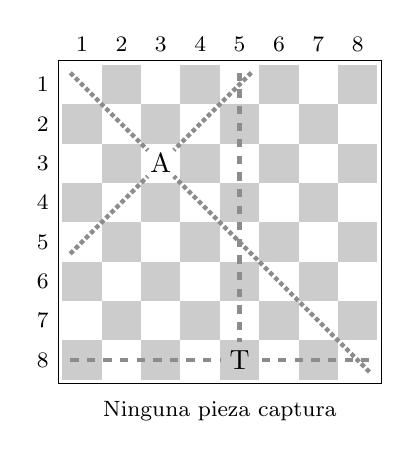
\begin{tikzpicture}[scale=.5, yscale=-1]
  \tablero
  \node[pieza] (alfil) at (3, 3) {A};
  \node[pieza] (torre) at (5, 8) {T};
  \draw[ma] (1 - .3, 1 - .3) -- (alfil);
  \draw[ma] (1 - .3, 5 + .3) -- (alfil);
  \draw[ma] (5 + .3, 1 - .3) -- (alfil);
  \draw[ma] (8 + .3, 8 + .3) -- (alfil);
  \draw[mt] (5     , 1 - .3) -- (torre);
  %\draw[mt] (5     , 8 + .3) -- (torre);
  \draw[mt] (8 + .3, 8     ) -- (torre);
  \draw[mt] (1 - .3, 8     ) -- (torre);
  \node at (4.5, 9.3) {\footnotesize Ninguna pieza captura};
\end{tikzpicture}

Escriba un programa que reciba como entrada
las posiciones en el tablero de un alfil y de una torre,
e indique cuál pieza captura a la otra:

\begin{minipage}[t]{.28\textwidth}
  \lstinputlisting[language=testcase,frame=single]{alfil-torre/caso2a.txt}
\end{minipage}
\hfil
\begin{minipage}[t]{.28\textwidth}
  \lstinputlisting[language=testcase,frame=single]{alfil-torre/caso2b.txt}
\end{minipage}
\hfil
\begin{minipage}[t]{.28\textwidth}
  \lstinputlisting[language=testcase,frame=single]{alfil-torre/caso2c.txt}
\end{minipage}

Suponga que todos los datos ingresados son válidos.
Su programa debe funcionar para tableros de \(1000\times 1000\).

